\def\year{2016}\relax
%File: formatting-instruction.tex
\documentclass[letterpaper]{article}
\usepackage{aaai16}
\usepackage{times}
\usepackage{helvet}
\usepackage{courier}
\usepackage{graphicx}
\usepackage{amsfonts}
\frenchspacing
\setlength{\pdfpagewidth}{8.5in}
\setlength{\pdfpageheight}{11in}
\pdfinfo{
/Title (Insert Your Title Here)
/Author (Put All Your Authors Here, Separated by Commas)}
\setcounter{secnumdepth}{0}  
 \begin{document}
% The file aaai.sty is the style file for AAAI Press 
% proceedings, working notes, and technical reports.
%
%\title{Formatting Instructions \\for Authors Using \LaTeX{}}
\title{Attention-based Sequence to Sequence Model for Tweet Normalization}
\author{AAAI Press\\
Association for the Advancement of Artificial Intelligence\\
2275 East Bayshore Road, Suite 160\\
Palo Alto, California 94303\\
}
\maketitle
\begin{abstract}
	Paraphrase identification for tweet is a new challenge due to informal expression. In this paper, we present a end-to-end approach to sequence learning that transfers text normalization into a neural machine translation task. Then a siamese recurrent architecture is used for learning sentence similarity after the sentences have been normalized. Our model employs a convolutional neural network and a highway network over characters, whose output is given to a long short-term memory recurrent neural network to map the input sequence to a vector of a fixed dimensionality, and then another long short-term memory to decode the target sequence from the vector. We add an attentional mechanism to improve the performance of tweet normalization, which can be beneficial to paraphrase detection indirectly. Novelty of this work is three-fold: First, to the best of our knowledge, this is an early attempt to adopt attention-based end-to-end model for tweet normalization. Second, our proposed model relies on	character-level inputs, making it fewer parameters to obtain comparable performance to word inputs. And third, we conduct a series of experiments and prove that the proposed method is advantageous over the state-of-art solutions for tweet normalization and semantic similarity. Our method shows significant performance gains on the paraphrase identification in tweet task compared with several strong baselines. 
\end{abstract}

\section{Introduction}
Semantic similarity of text are used in many semantic tasks such as paraphrase identification \cite{Xu-EtAl-2014:TACL}, textual entailment \cite{henderson-popa:2016:P16-1}, and question answering \cite{Severyn:2015:LRS:2766462.2767738}. Twitter engages millions of users, who naturally talk about the same topics simultaneously and frequently convey similar meaning using diverse linguistic expressions. The unique characteristics of this user-generated text presents new challenges and opportunities for semantic similarity measurement. Unfortunately, traditional natural language processing methods sometimes perform poorly when processing this kind of text. One reason is that tweets are very informal, and contain many misspelled words, abbreviations and many other non-standard tokens, which make it substantially different from formal written text. To improve the performance on the social media semantic similarity, it is inevitable to leverage normalization techniques which can automatically convert the non-standard tokens into the corresponding standard words.

Intuitively, tweet normalization will be beneficial for paraphrase identification and textual  semantic similarity. For example, if `tmr' is converted to `tomorrow', it will improve the semantic representation for tweets and promote similarity comparison performance between text pairs. This normalization task has received an increasing in social media language processing. However, most of previous work on normalization assumed that they already knew which tokens are non-standard words (NSW) that need normalization. Then different methods are applied only to these tokens. Han and Baldwin \shortcite{han-baldwin:2011:ACL-HLT2011} is the typical work which made a pilot reasearch on NSW identification. One straight forward method to do this is to use a dictionary to classify a token into in-vocabulary (IV) words and out-of-vocabulary (OOV) words, and just treat all the OOV words as NSW. Contrast to straight forward work, joint part-of-speech (POS) and text normalization was proposed by Li and Liu \shortcite{Li:2015:JPT:2832415.2832425}, the objective of this work is to perform POS tagging and text normalization at the same time. It indicates the thought that joint tweet normalization and similarity.

Character-aware neural language model \cite{Kim-AAAI1612489} relies only on character-level inputs and predictions are still made at the word-level, and the model can leverage subword information through a character-level convolutional neural network (CNN) and have a good performance on the estimation of rare words embeddings. Therefore, it is attracting to explore neual language model for tweet normalization. Xu et al. \shortcite{xu-callisonburch-dolan:2015:SemEval} proposed a share task evaluation on both  paraphrase identification and semantic textual similarity for Twitter data. Although some works \cite{zarrella-EtAl:2015:SemEval,vandergoot-vannoord:2015:SemEval} take tweet normalization into account, this researches are limited to replace the OOV words with normalization dictionary.

In this paper, we proposed a character-level neural language model for tweet normalization, and then measure the semantic of normalized text for paraphrase identification and textual similarity. Our work investigates two methods using normalized tweets for sematic similarity measurement. One adopts a pipline strategy, and the other uses a joint fashion. Our experimental results demonstrate that our proposed model gives a significant performance improvement on NSW detection compared with the dictionary baseline system and our proposed joint model performs better than the pipeline method, and it outperforms the state-of-the-art paraphrase identification system. To summarize, our contributions in this paper are as follows:

\begin{itemize}
	\item We proposed a character-level neural language model for tweet normalization, which achieve results on par with the existing state-of-the-art NSW detection.
	\item The proposed joint model can combine the normalization and semantic textual similarity techniques to improve the fprmance of these two tasks on English social media data.
	\item We demonstrate the effectiveness of our proposed method. Experimental results achieve the state-of-the-art performance on normalization and similarity.
\end{itemize}

\section{Model}
The proposed model adopt a sequence to sequence method for learning a neural language model. We illustrate these two model types in Figure 1.
\begin{figure}
\centering
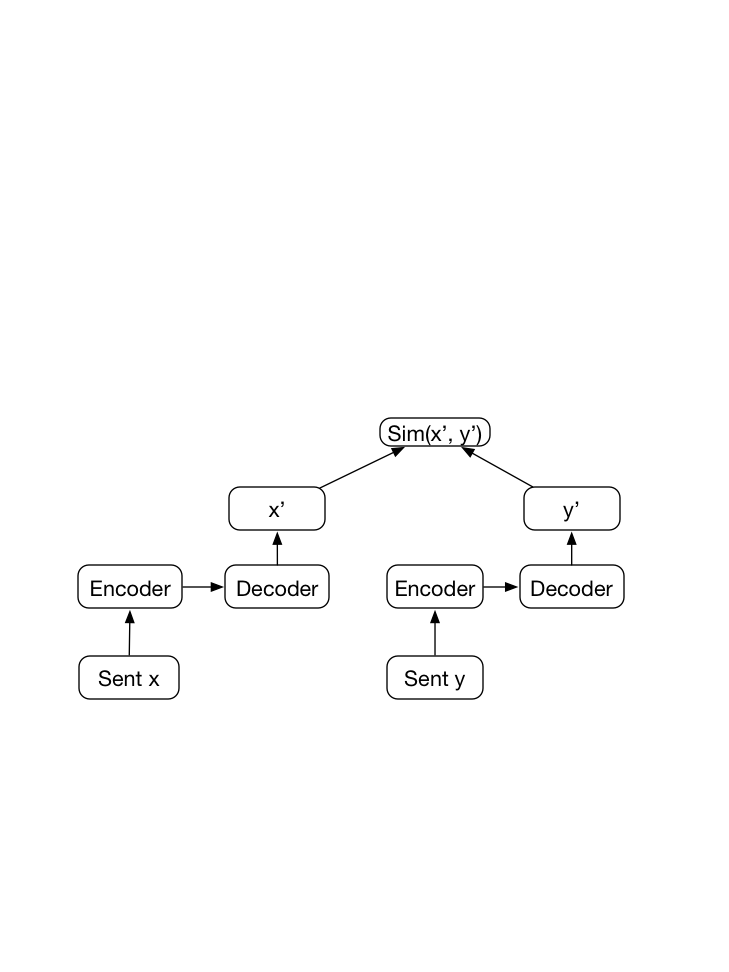
\includegraphics[width=0.7\linewidth]{model}
\caption{The structure of model}
\label{fig:model}
\end{figure}


The model includes two parts, one is normalization, and other is similarity.

The question that inspired this paper was whether neural language model could also benefit for text normalization.; that is ... To answer this question we introduce character-aware neural language model for tweets normalization.  \textbf{Draw the figure of model.}

\subsection{Long Short-Term Memory}
Recurrent neural networks (RNNs) are able to process input sequences of arbitrary length via the recursive application of a transition function on a hidden state vector \textit{$h_{t}$}. At each time step \textit{t}, the hidden state \textit{$h_{t}$} is a function of the input vector \textit{$x_{t}$} that the network receives at time \textit{t} and its previous hidden state \textit{$h_{t-1}$}. The hidden state \textit{$h_{t}$} $\in$ $\mathbf{R^{d}}$ can be interpreted as a \textit{d}-dimensional distributed representation of the sequence of tokens observed up to time \textit{t}. Commonly, the RNN transition function is an affine transformation followed by a pointwise non-linearity such as the hyperbolic tangent function:
\begin{equation}\label{rnn}
h_{t} = \tanh(Wx_{t}+Uh_{t-1}+b)
\end{equation}
However, a problem with RNNs with transition functions of this form is that during traning , components of the gradient vector can grow or decay exponentially over long sequences \cite{Hochreiter:1998:VGP:353515.355233}. This problem with exploding or vanishing gradients makes it difficult for the RNN model to learn long-distance correlations in a sequence.

The LSTM architecture addresses this problem of learning long-term dependencies by introducing a memory cell that is able to preserve state over long periods of time \cite{Hochreiter:1997:LSM:1246443.1246450}. While numerous LSTM variants have been described, here we describe the version used by Zaremba and Sutskever \shortcite{DBLP:journals/corr/ZarembaS14}. We define the LSTM unit at each time step \textit{t} to be a collection of vectors in \textbf{$R^{d}$}: an input gate \textit{$i_{t}$}, a forget gate \textit{$f_{t}$}, an output gate \textit{$o_{t}$}, a memory cell \textit{$c_{t}$} and a hidden state \textit{$h_{t}$}. The entries of the gating vectors \textit{$i_{t}$}, \textit{$f_{t}$} and \textit{$o_{t}$} are in [0, 1]. We refer to \textit{d} as the memory dimension of the LSTM. The LSTM transition equations are the following:
\begin{equation}\label{lstm-i}
i_{t} = \sigma(W^{(i)}x_{t}+U^{(i)}h_{t-1}+b^{(i)})
\end{equation}
\begin{equation}\label{lstm-f}
f_{t} = \sigma(W^{(f)}x_{t}+U^{(f)}h_{t-1}+b^{(f)})
\end{equation}
\begin{equation}\label{lstm-o}
o_{t} = \sigma(W^{(o)}x_{t}+U^{(o)}h_{t-1}+b^{(o)})
\end{equation}
\begin{equation}\label{lstm-u}
u_{t} = \tanh(W^{(u)}x_{t}+U^{(u)}h_{t-1}+b^{(u)})
\end{equation}
\begin{equation}\label{lstm-c}
c_{t} = i_{t} \odot u_{t} + f_{t} \odot c_{t-1}
\end{equation}
\begin{equation}\label{lstm-h}
h_{t} = o_{t} tanh(c_{t})
\end{equation}
where \textit{$x_{t}$} is the input at the current time step, $\sigma$ denotes the logistic sigmoid function and $\odot$ denotes elementwise multiplication. Intuitively, the forget gate controls the extent to which the previous memory cell is forgotten, the input gate controls how much each unit is updated, and the output gate controls the exposure of the internal memory state. The hidden state vector in an LSTM unit is therefore a gated, partial view of the state of the unit's internal memory cell. Since the value of the gating variables vary for each vector element, the model can learn to represent information over multiple time scales.

\subsection{Neural Language Model}
The goal of the LSTM is to estimate the conditional probability \textit{p}(\textit{$y_{1},...,y_{T^{'}}|x_{1},...,x_{T}$}) where (\textit{$x_{1},...,x_{T}$}) is an input sequence and \textit{$y_{1},...,y_{T^{'}}$} is its corresponding output sequence whose length \textit{$T^{'}$} may differ from \textit{T}. The LSTM computes this conditional probability by first obtaining the fixed-dimensional representation \textit{v} of the input sequence (\textit{$x_{1},...,x_{T}$}) given by the last hidden state of the LSTM, and then computing the probability of \textit{$y_{1},...,y_{T^{'}}$} with a standard LSTM language model formulation whose initial hidden state is set to the representation \textit{v} of \textit{$x_{1},...,x_{T}$}:
\begin{equation}\label{nlm}
p(y_{1},...,y_{T^{'}}|x_{1},...,x_{T})=\prod_{t=1}^{T^{'}}p(y_{t}|v,y_{1},...,y_{t-1})
\end{equation}
In this equation, each \textit{p($y_{t}|v,y_{1},...,y_{t-1}$)} distribution is represented with a softmax over all the words in the vocabulary. Note that we require that each sentence ends with a special end-of-sentence symbol ``$<$EOS$>$", which enables the model define a distribution over sequences of all possible lengths.

\subsection{Attention-Based Encoder }
Attention-based contextual encoder that constructs a representation based on the generation context. Attention models adopt a look-back strategy by linking the current decoding stage with input sentences in an attempt to consider which part of the input is most responsible for the current decoding state. 

Let \textit{H}= \{$h_{1}^{s}(e)$, $h_{2}^{s}(e)$, ..., $h_{N}^{s}(e)$\} be the collection of sentence-level hidden vectors for each sentence form the inputs, outputed from LSTM sentence encoder. Each element in \textit{H} contains information about input sequences with a strong focus on the parts surrounding each specific sentence (time-step). During decoding, suppose that \textit{$e_{t}^{s}$} denotes the sentence-level embedding at current step and that \textit{$h_{t-1}^{s}$}(dec) denotes the hidden vector outputted from LSTM sentence decode at previous time step \textit{t}-1. Attention models would first link the current step decoding information, i.e., \textit{$h_{t-1}^{s}$}(dec) which is outputted form LSTM with each of the input sentence \textit{i} $\in$ [1, \textit{N}], characterized by a strength indicator \textit{$v_{i}$}:
\begin{equation}\label{key}
v_{i} = U^{T}f(W_{1} \cdot h_{t-1}^{s}(dec) + W_{2} \cdot h_{i}^{s}(enc))
\end{equation}
\textit{$W_{1}$}, \textit{$W_{2}$} $\in$ $\mathbb{R}^{K \times K}$, \textit{U} $\in$ $\mathbb{R}^{K \times 1}$. \textit{$v_{i}$} is then normalized:
\begin{equation}\label{key}
a_{i}=\frac{\exp(v_{i})}{\sum_{i^{'}}\exp(v_{i}^{'})}
\end{equation}
The attention vector is then created by averaging weights over all input sentences:
\begin{equation}\label{key}
m_{t}=\sum_{i \in [1, N_{D}]}a_{i}h_{i}^{s}(enc)
\end{equation}
LSTM hidden vectors for current step is then achieved by combining \textit{$c_{t}$}, \textit{$e_{t}^{s}$} and \textit{$h_{t-1}^{s}$}(dec):

\begin{equation}\label{key}
c_{t} = f_{t} \cdot c_{t-1} + i_{t} \cdot l_{t}
\end{equation}
\begin{equation}\label{key}
h_{t}^{s} = o_{t} \cdot c_{t}
\end{equation}
where \textit{W} $\in$ $\mathbb{R}^{4K \times 3K}$. \textit{$h_{t}$} is then used for word predicting as in the vanilla version of the hierarchical model.

\subsection{Training}
The lack of generation constrants makes it posible to train the model on arbitrary input-output pairs. Once we have defined the local conditional model, \textit{$p$}($y_{i+1}$$|$x, $y_{c}$; $\theta$), we can estimate the parameters to minimize the negative log-likelihood of a set of summaries. Define this training set as consisting of \textit{N} input-output pairs ($\textbf{x}^{(1)}$, $\textbf{y}^{(1)}$),...,($\textbf{x}^{(N)}$, $\textbf{y}^{(N)}$). The negativ log-likelihood conveniently factors into a term for each token in the decode sentence:
\begin{equation}\label{key}
NLL(\theta)=-\sum_{j=1}^{J}\log p(\mathbf{y}^{(j)}|\mathbf{x}^{(j)};\theta)
\end{equation}
We minimize NLL by using mini-batch stochastic gradient descent.

\subsection{Attention}
In parallel, the concept of ``attention" has gained popularity recently in training neural networks, allowing models to learn alignments between different modalities. In the context of NMT, Bahdanaul et al. \shortcite{DBLP:journals/corr/BahdanauCB14} as successfully applied such attentional mechanism to jointly translate and align words. To the best of our knowledge, there has not been any other work exploring the use of attention-based architectures for NMT.

Word, Character, attention, sequence to sequence, language model, tweet normalization, semantic similarity, end-to-end.

\subsection{Normalization}
Given a piece of microtext, our model will normalize terms one bye one. Thus, the challenge is to determine the corresponding standard form \textit{t}, which can be a term or a sequence of terms, for each observed term \textit{t'}. Notice that \textit{t} many or may not be the same with \textit{t'}. \textit{t'} is a NSW if \textit{t'} $\neq$ \textit{t}. Thus, the task is to find the most probable normalization \textit{t*} for each observed term \textit{t'}:
\begin{equation}\label{key}
t*=argmax_{t}P(t|t')=argmax_{t}P(t'|t)P(t)
\end{equation}
P(t'$|$t) models the noisy channel through which an intended term \textit{t} is sent and is corrupted into the observed term \textit{t'}. P(t) models the source that generates the intended term \textit{t}. In practice, the source model can be approximated with an n-gram statistical language model.

Since a non-standard term and its corresponding standard form might be similar from one or multiple perspective(s), it is reasonable to assume that there are several channels, each of which would distort an intended term in one of the above aspects. More specifically, a grapheme channel would be responsible for the spelling distortion, a phoneme channel would cause phonetic corruptions, a context channel may shrink a sequence of terms into one term. In reality, an intended word may be transferred through one or multiple channels, and an observed term might be mixed corruption from more than one channel. Under this assumption, and letting \{\textit{$c_{k}$}$|$\textit{$c_{k} \in C$}\} denotes the set of channels, so the aforementioned equation can be further developed to 
\begin{equation}\label{key}
t*= argmax_{t}\sum_{k}P(t',c_{k}|t)P(t)
  = argmax_{t}\sum_{k}P(t'|c_{k},t)P(c_{k}|t)P(t)
\end{equation}
A term \textit{t} is transfered through channel \textit{$c_{k}$} with probability P($c_{k}|$t). Within the channel \textit{$c_{k}$}, term \textit{t} is distorted to term \textit{t}' according to the channel model P(t'$|c_{k}$, t).

Many approaches to text normalization adopt the noisy channel setting, where the model normalization source sentence \textit{s} into target canonical form \textit{t} is factored into two parts $\hat{t}$ = argmax$_{t}$\textit{P}(\textit{t})\textit{P}(\textit{s}$\vert$\textit{t}). The error term \textit{P}(\textit{s}$\vert$\textit{t}) models hwo canonical strings are transformed into variants such as misspellings or abbreviations. The language model \textit{P}(\textit{t}) encodes which target strings are probable. When large-scale normalized texts have been trained with language model, the weights of the model are obtained with the normalization corpus. When the informal texts are inputed into model, the decoder of the proposed model will output the normalized text sequence and the informall words will be changed following the context information, which will be expressed with normalized words form normalized corpus dictionary. \textbf{AAAI2011Normalizing Microtext}

\subsection{Similarity Measurement}
We adopt a siamese architecture for learning sentence similarity. There are two networks LSTM$_a$ and LSTM$_b$ which each process one of the sentences in a given pair, but our networks architecture tied weights such that LSTM$_a$ equals LSTM$_b$ in this work. Nevertheless, the general united version of this model may be more useful for applications with asymmetric domains such as information retrieval. The LSTM learns a mapping from the space of variable length sequences of d$_in$-dimensional vectors into $\mathbb{R}^{d_{rep}}$. More concretely, each sentence (represented as a sequence of word vectors) \textit{$x_{1},\cdots,x_{T}$}, is passed to the LSTM, which updates its hidden state at each sequence-index. The final representation of the sentence is encoded by \textit{$h_{T}$} $\in$ $\mathbb{R}^{d_{rep}}$, 
the last hidden state of the model. For a given pair of sentences, our approach applies a pre-defined similarity function \textit{g}: $\mathbb{R}^{d_{rep}}\times\mathbb{R}^{d_{rep}}\rightarrow\mathbb{R}$ to their LSTM-representations. Similarites in the representation space are subsequently used to infer the sentences' underlying semantic similarity.

Note that unlike typical language model RNNs, which are used to predict the next word given the previous text, our LSTMs simply function like the encoder of sequence to sequence model. Thus, the sole error signal backpropagated during training stems from the similarity between sentence representations \textit{$h_{T_{a}}^{(a)}$}, \textit{$h_{T_{b}}^{(b)}$}, and how this predicted similarity deviate from the human annotated ground truth relatedness. We restrict ourselves to the simple similarity function: (\textit{subscript must be changed as $h_{T_{1}}^{(1)}$}, or it is same as SiamStru(AAAI16).)
\begin{equation}\label{key}
sim(h_{T_{a}}^{(a)},h_{T_{b}}^{(b)}) = \exp(-||h_{T_{a}}^{(a)}-h_{T_{b}}^{(b)}||_{1}) \in [0,1]
\end{equation}
This forces the LSTM to entirely capture the semantic difference during training, rather than supplementing the RNN with a more complex learner that can help resolve shorcoming in the learned representations.

\section{Experiments}
We evaluated our model on the tweet normalization and paraphrase identification task, which is a benchmark for evaluating many semantic similarity models.

\subsection{Dataset}
The following data sets are used in our experiments. It includes tweet normalization and paraphrase identification.

\begin{itemize}
	\item Data 1: 2,333 unique pairs of informal tokens and normalized words, collected form 2,577 Twitter messages, which selected form the Edinburgh Twitter corpus \cite{pennell-liu:2011:IJCNLP-2011}. And some changes were made on this data\footnote{http://www.hlt.utdallas.edu/~chenli/normalization} by Li and Yang \shortcite{li-liu:2014:P14-3}. This data is used for training the normalization models for tweet normalization.
	\item Data 2: The data\footnote{http://www.hlt.utdallas.edu/~chenli/normalization\underline{ }pos/} was created by Chen and Liu \shortcite{Li:2015:JPT:2832415.2832425}, which is used for joint POS tagging and normalization of non-standard tokens. The data contains two parts: one is from, which includes 549 tweets. The another contains 789 tweets. We removed the POS tagging and use the first as test data and the second as valid data.
	\item Data 3: We use the PIT corpus\footnote{http://www.cis.upenn.edu/~xwe/
	semeval2015pit/} for evaluating paraphrase identification. The training and development set contain 17,790 sentence pairs and test set includes 972 sentence pairs\cite{xu-callisonburch-dolan:2015:SemEval}. The data set can be used for paraphrase identification and semantic similarity in Twitter.
\end{itemize}

\subsection{Traing Detail}
Existing research has shown that attention mechanism work better than shallow recurrent neural network for squence to sequence tasks \cite{luong-pham-manning:2015:EMNLP,Sutskever:2014:SSL:2969033.2969173}. We adopt attention-based end-to-end structure with three layer for encoding and three layer for decoding, each of which is comprised of a different set of parameters. Each LSTM layers consists of 500 hidden neurons and the dimensionality of word embeddings is set to 500. Some other training details given as following.

\begin{itemize}	
	\item Input sentence sequences are reversed.
	\item Parameters are initialized form a uniform distribution between [-0.1, 0.1].
	\item Batch size is set to 16.
	\item Stochastic gradient descent is implemented without momentum using a fixed learning rate of 1. We start halving the learning rate every half epoch after 5 epochs. We trained our models for a total of 20 epoches.
	\item Dropout rate is set to 0.3.
	\item Size of the character embeddings is set to 30.
	\item Number of covolution filters is 500.
\end{itemize}

Our implementation on a single GPU\footnote{The GPUs with 1280 Cuda cores and 6GB memory.} processes a speed of approximately 5,000-6,000 tokens per second.

\subsection{Results}
A summay of our experimental results for tweet normalization is given Table 1. We observe better performances for tweet normalization based on character-level input than the word-level with attention mechanism. In the Table, the experimental results include two parts input: word-level (Word) and character-level (Char). In each method, we use LSTM, attention (Attn) and reverse the source sequence (Rev), which is crucial to achieving good performance \cite{Sutskever:2014:SSL:2969033.2969173}. However, pre-trained word embeding is blind to subword information, and representation of rare words can be poorly estimated, leading to high perplexities for rare words. This is especially problematic in morphologically rich languages with long-tailed frequency distribution of domains with dynamic vocabularies (e.g. Twitter). So we adopta character-level convolutional neural networks for leverages subword infomration, which output is used as an input to a long short-term memory network. Similar to the memory cells in LSTM networks, highway (HW) layers allow for training of deep networks by adaptively carrying some dimensions of the input directly to the output. In our method, a max-over-time pooling operation is applied to obtain a fixed-dimensional representation of the word, which is given to the highway network. The highway network' output is used as the input to LSTM. From the table 1, we observe that the proposed method can obtain the comparable performance to joint decoding for tweet normalization. In addition, the character-level input has significant performance on word-level embedding input. Meanwhile, the attentional mechanism is beneficial to sequence to sequence model.
\begin{table}
	\begin{center}
		\begin{tabular}{| c | c | c | }
			\hline
			\bf Method & \bf Accuracy \\ \hline
			First-order Markov Viterbi & 0.761 \\ \hline
			Secod-order Markov model & 0.770 \\ \hline
			Joint Decoding & \textbf{0.773} \\ \hline
			Word+LSTM & 0.714 \\ \hline
			Word+LSTM+Rev & 0.725   \\ 
			\hline
			Word+LSTM+Attn & 0.732   \\ 
			\hline
			Word+LSTM+Rev+Attn & 0.746   \\ 
			\hline
			Char+CNN+LSTM & 0.742   \\ 
			\hline
			Char+CNN+HW+LSTM & 0.751   \\ 
			\hline
			Char+CNN+HW+LSTM+Rev & 0.765   \\ 
			\hline
			Char+CNN+HW+LSTM+Rev+Attn & 0.771 \\ 
			\hline
		\end{tabular}
		\caption{Tweet normalization results on test set.}
	\end{center}
\end{table}

After tweet normalization, the model has capability for normalizing the informal text. So we utilize the model with same parameters and weight for similarity evaluation. Both paraphrase identification and semantic similarity are used for evaluating the performance of tweet normalization. The paraphrase identification results are presented in Table 2. There are precesion(\textit{Prec}), recall(\textit{Rec}) and F-measure(\textit{$F_{1}$}) for evaluating the performance of proposed model. There are four baselines, including logistic regression \cite{das-smith:2009:ACLIJCNLP}, weighted matrix factorization \cite{guo-diab:2012:ACL2012}, referential machine translation \cite{bicici:2015:SemEval} and recursive auto-encoder \cite{NIPS2011_4204}. From the Table 2, we conclude that our method with character-level (Char) input is better than word-level (Word) input on paraphrase detection and the methods with normalization (Norm) have higher \textit{$F_{1}$} than the methods without normalization. What is more, our four methods obtain significant performance than other four baselines. The results indicates that normalization can promote the semantic representation of informal text.

\begin{table}
	\begin{center}
		\begin{tabular}{| c | c | c | c | }
			\hline
			\bf Methods & \bf \textit{Prec} & \bf \textit{Rec}  &\bf  \textit{F}$_{1}$ \\ \hline
			Logistic Regeression  & 0.679 & 0.520 & 0.589  \\ \hline
			Recursive Auto-encoder  & 0.543 & 0.394 & 0.457  \\ 
			\hline
			Weighted Matrix Factorization & 0.450 & 0.663 & 0.536  \\ 
			\hline
			Referential Machine Translation  & 0.859 & 0.417 & 0.562  \\ 
			\hline
			Our Method (Word) without Norm& 0.598 & 0.631 & 0.614  \\ 
			\hline
			Our Method (Word) with Norm & 0.642 & 0.651 & 0.646  \\ 
			\hline
			Our Method (Char) without Norm & 0.637 & 0.649 & 0.643  \\ 
			\hline
			Our Method (Char) with Norm & 0.654 & 0.672 & \bf 0.663  \\ 
			\hline
		\end{tabular}
		\caption{Test set results on PIT for paraphrase identification.}
	\end{center}
\end{table}

We also implement semantic similarity experiment on PIT, the results are given in Table 3, the pearson is used for semantic similarity. As the same as the paraphrase identification, we adopt four method, including word-level and character-level input with optional tweet normalization, for evaluating the performance of the proposed methods. In addition, we also use four baselines, including logistic regeression \cite{das-smith:2009:ACLIJCNLP}, Two-layer Neural Network \cite{bertero-fung:2015:SemEval}, Weighted Matrix Factorization \cite{guo-diab:2012:ACL2012} and Recurrent Neural Network \cite{zarrella-EtAl:2015:SemEval} for comparing the experimental performance. From the Table 3, we conclude that our model adopted the character-level input with normalization obtains the highest pearson score and word-level input also has better performance than other four baseline methods.

\begin{table}
	\begin{center}
		\begin{tabular}{| c | c | c | }
			\hline
			\bf Model & \bf \textit{Pearson}  \\ \hline
			Logistic Regeression  & 0.511   \\ \hline
			Two-layer Neural Network  & 0.545   \\ 
			\hline
			Weighted Matrix Factorization  & 0.350   \\ 
			\hline
			Recurrent Neural Network  & 0.619   \\ 
			\hline
			Our Method (Word) without Norm  & 0.581   \\ 
			\hline
			Our Method (Word) with Norm  & 0.604   \\ 
			\hline
			Our Method (Char) without Norm & 0.613   \\ 
			\hline
			Our Method (Char) with Norm  & \bf 0.628  \\ 
			\hline
		\end{tabular}
		\caption{Test set results on PIT for semantic similarity.}
	\end{center}
\end{table}

\section{Related Work}
Neural language models (NLM) contain a rich family of neural network architectures for language modeling. Some examples encompass recurrent \cite{mikolov2010recurrent}, convolutional \cite{wang-EtAl:2015:ACL-IJCNLP3}, and convolutional-recurrent \cite{Kim-AAAI1612489}. In Twitter, there are existing rare and unknown words due to the social media characteristic,  therefore it is necessary for language model to point the unknown words before normalization. A neural network models using attention adopted two softmax layers in order to predict the next word in conditional language models \cite{gulcehre-EtAl:2016:P16-1}. Recurrent memory network \cite{tran-bisazza-monz:2016:N16-1} not only amplifies the power of recurrent neural networks but also facilitates the understanding of its internal functions, the model can learn the correct words by the trained language model. Log-bilinear language models integrate compositional morphological representations and probabilistic language modelling \cite{jan-phil:2014:icml}.

Character-aware neural language model \cite{Kim-AAAI1612489} can capture morphological features based on character-level input and the output is still word-level. Because the social media has long-tailed frequency distributions or domains with dynamic vocabularies, so the model can leverage subword information for tweets normalization. The existing works for semantic similarity focus on sequence representation, and the model structure is usually a siamese architecture, which represent sentence pairs and compute the semantic similarity between pairs \cite{jonas-aditya:2016:AAAI}. Convolutional neural networks are used for representing sentence and learn multigranular sentence representations for paraphrase identification was proposed \cite{yin-schutze:2015:NAACL}. The deep learning architecture based on convolutional networks can obtain mutliple levels of granularity, including unigram, short-ngram, long-ngram and sentence-level features, which are computed for similarity comparation for paraphrase detection.

Although normalization on informal text has potential function on sentence representation and semantic similarity, paraphrase can also improve the normalization performance \cite{ling-EtAl:2013:EMNLP} on parallel microblog data. Applying alignment feature for semantic similarity of text can capture both local ifnormation like lexical semantics and structural information like syntactic structures \cite{chen-praveen:2016:ijcai}. The method can avoid conventional fixed-length sentence representation and add more feature information for similarity measurement. Some works \cite{DBLP:journals/corr/WietingBGL15a,pavlick-EtAl:2015:ACL-IJCNLP} consider the utilization of paraphrse database \cite{ganitkevitch-vandurme-callisonburch:2013:NAACL-HLT,pavlick-EtAl:2015:ACL-IJCNLP3}for sentence similarity, entialment, and sentiment classification.

Our work apply character-level input style convolutional recurrent neural network model for trianing a language model on word-level prediction. After pre-trained with formal corpus such as Wiki or Penn Treebank data, the language model is used for normalizing the informal tweets, which can automatically point unknown or non-standard words and normalize them. The normalized tweets will be measured semantic similarity further, and the similarity will feedback for normalization based on assumptaion that paraphrasing sentence pairs will keep semantic equivalence. The experimental results demonstrate that our model outperform the existing state-of-the-art systems.

\section{Conclusion}
In this paper, we proposed a novel approach for tweet normalization and semantic similarity. The proposed method adopted a sequence to sequence model with attention-based mechanism, which is used for tweet normalization. After normalized text, the model with pre-trained is used for paraphrase identification and sematic similarity. Our model leverages subword information through a character-level convolutional neural network which output is used as an input to a recurrent neural network, and it is beneficial to morphologically rich languages with long-tailed frequency distribution or domains with dynamic vocabularies. A max-over-time pooling operation for convolutional neural networks is applied to obtain a fixed-deimensional representation of word, which is given to a highway network. The highway network's output is used as the input to long short-term memory. The encoder encodes a variable source sequence to a fixed dimensional representation and decoder decodes the representation to a variable target sequence. The end-to-end model normalizes informal text, and the pre-trained model is used for sentence semantic representation further. We test the effectiveness of our models in the paraphrase identification and semantic similarity in Twitter. Our attention-based character-level input method yields large gains over non-attention models for the paraphrase identification and semantic similarity. In the future, we plan to apply the proposed methods for question answer tasks in social media.

\bibliographystyle{aaai}
\bibliography{aaai16.bib}

\end{document}
